\documentclass[ngerman]{beamer}

%style
\mode<presentation>{
	\usetheme{Goettingen}
	%\usetheme{default}
}
%packages
\usepackage[utf8]{inputenc}
\usepackage[ngerman]{babel}
\usepackage{graphicx}

%
% packages.tex -- zusätzliche Packages 
%
% In diesem File werden \usepackage{}-Aufrufe eingetragen für Packages, die
% noch nicht im skript.tex aufgerufen werden
%
% (c) 2018 Hansruedi Patzen, Hochschule Rapperswil
%



%Einstellungen Präsentation
\title{Klima auf anderen Planeten}
\author{Nicolas Tobler}
\institute{Mathematisches Seminar 2018}
\date{14.05.2018}

%Bilder
\graphicspath{{Pictures/}}

%Beginn der Präsentation
\begin{document}

%Titelseite
\begin{frame}
\titlepage
\end{frame}

%Inhaltsverzeichnis
\begin{frame}
\frametitle{Inhalt}
\tableofcontents
\end{frame}

\section{Einführung}

\subsection{Planeten im Vergleich}
\begin{frame}
	\frametitle{Planeten im Vergleich}
	
	\begin{figure}
	\center
	\includegraphics[width=0.7\linewidth, trim={0 3cm 0 3cm},clip]{planets.jpg}
	\end{figure}
	
\begin{center}
\begin{tabular}{ l c r }
	%\hline
  Mars & Erde & Venus \\
  \hline
  Kaum Wolken & Moderates Wetter & Dicke Wolkendecke \\
  Kalt & Mild & Heiss \\
	%\hline
\end{tabular}
\end{center}	
	
%	
%\begin{columns}
%\begin{column}{0.33\textwidth}
%   Mars
%   \begin{itemize}
%   		\item[-] Kaum Wolken
%   		\item[-] Heiss
%   \end{itemize}
%\end{column}
%\begin{column}{0.33\textwidth}
%   Venus
%   \begin{itemize}
%   		\item[-] Dicke Wolkendecke
%   		\item[-] Heiss
%   \end{itemize}
%\end{column}
%\begin{column}{0.33\textwidth}
%   Erde
%   \begin{itemize}
%   		\item[-] Normales Wetter
%   \end{itemize}
%\end{column}
%\end{columns}

\end{frame}

\subsection{Ziele}
\begin{frame}
\frametitle{Ziele}
\begin{itemize}

	\item[$\bullet$] Ziele
	\begin{itemize}
		\item[-] Klima mit Planet-Eigenschaften verknüpfen
		\item[-] Werdegang der Planeten nachvollziehen
	\end{itemize}

	\item[$\bullet$] Idee
	\begin{itemize}
		\item[-] Planeten mit gleichem Modell simulieren
		\item[-] Orbitale Eigenschaften verwenden
	\end{itemize}

\end{itemize}
\end{frame}

\subsection{Vorgehen}
\begin{frame}
\frametitle{Vorgehen}
\begin{itemize}

	\item[$\bullet$] Für alle Planeten geltendes Modell  erstellen
	\item[$\bullet$] Annahmen
	\begin{itemize}
		\item[-] Gleiche materielle Eigenschaften
		\item[-] Gleiches Vorkommen an Wasser
		\item[-] Wasser hat grösste Auswirking auf Klima
	\end{itemize}
	
	\item[$\bullet$] Freie Parameter abschätzen
\end{itemize}
\end{frame}


\section{Modell} 
\begin{frame}
	\frametitle{Modell}
	\begin{figure}
		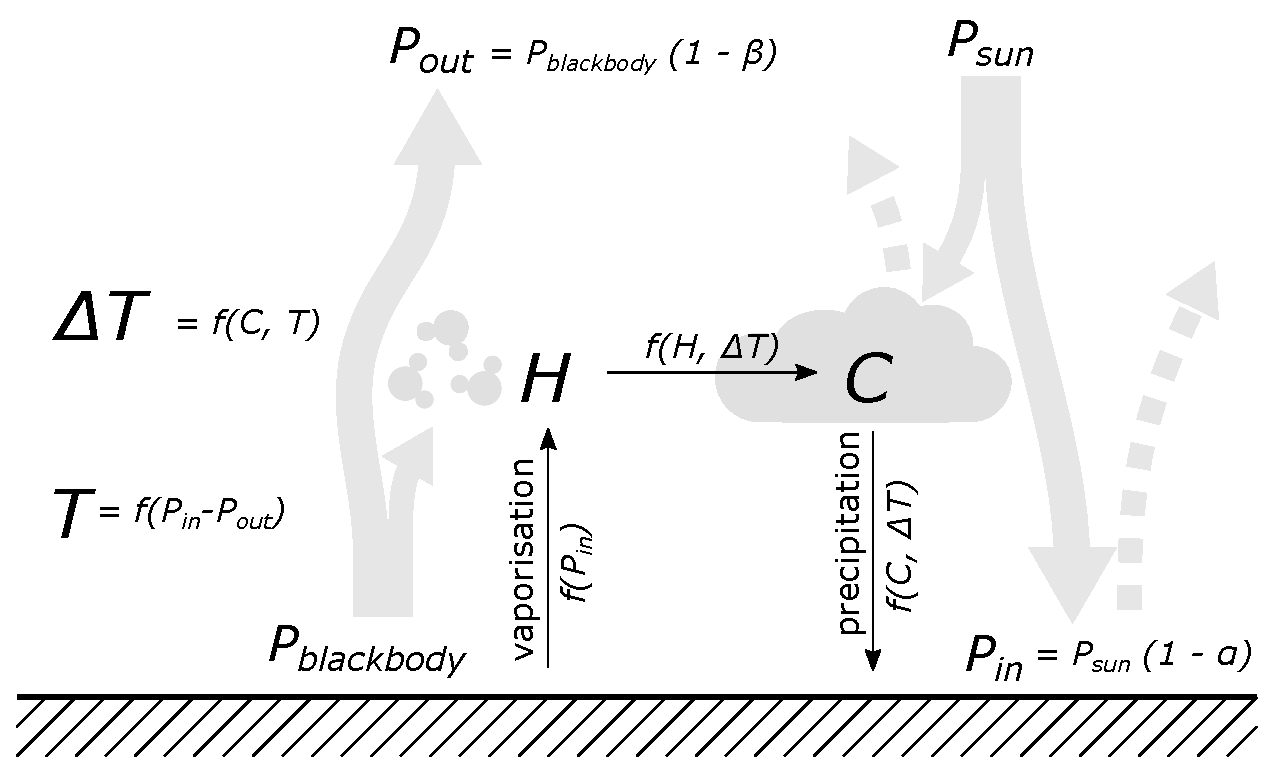
\includegraphics[width=\linewidth]{Model.eps}
	\end{figure}
\end{frame}

\subsection{Energiehaushalt}
\begin{frame}
\frametitle{Energiehaushalt}
\begin{itemize}
	\item[] Absorbierte Leistung
	\begin{equation}
	P_{in} = \sigma T_{\astrosun}^4 \left( \frac{R_{\astrosun}}{A_{planet}} \right) ^2 \cdot (1-\alpha)
	\end{equation}
	\pause
	
	\item[] Abgestrahlte Leistung
	\begin{equation}
	P_{out} = (4 \pi R^2 \sigma T^4)(1 - \beta)
	\end{equation}
	\pause
	
	\item[] Albedo
	\begin{equation}
	\alpha(C) = (0.55 \cdot C) + 0.10;
	\end{equation}
	\pause
	
	\item[] Treibhauseffekt
	\begin{equation}
	\beta(H) = 0.6 \cdot H
	\end{equation}
\end{itemize}
\end{frame}




\subsection{Wasserkreislauf}

\begin{frame}
	\frametitle{Wasserkreislauf}
	\begin{itemize}
		\item[] Wasserdampfbildung
			\begin{equation}
			\xi_4 (P_{in})
			\end{equation} 
		\pause
		\item[] Wolkenbildung
			\begin{equation}
			\xi_5 \left( H \frac{dT}{dh} \right)
			\end{equation}
		\pause
		\item[] Wolkenabbau 
		 	\begin{equation}
			\xi_6 (C)
			\end{equation}
	\end{itemize}
\end{frame}

\begin{frame}
	\frametitle{Wasserkreislauf}
	\begin{itemize}
	
		\item[] Wasserkreislauf
			\begin{equation}
				\begin{matrix}			
					\dot{H} = & \xi_4 P_{in}(C) & - \xi_5  H \frac{dT}{dz} & \\
					\dot{C} = &                 &   \xi_5  H \frac{dT}{dz} & - \xi_6 C
				\end{matrix}	
			\end{equation}
	
		\item[] Temperaturgradent
			\begin{equation}
				\frac{dT}{dz} \approx \Delta T
			\end{equation}
		
		\item[] Eingesetzt
			\begin{equation}
				\begin{matrix}			
					\dot{H} = & \xi_4 P_{in}(C) & - \xi_5 H \Delta T & \\
					\dot{C} = &                 &   \xi_5 H \Delta T & - \xi_6 C
				\end{matrix}	
			\end{equation}			
		
	\end{itemize}
\end{frame}

\subsection{Temperaturgradient}

\begin{frame}
	\frametitle{Temperaturgradient}
	\begin{itemize}
	
		\item[]Wasser kondensiert  $\rightarrow$ Niedriger Gradient
		
		\item[]Wärmere luft $\rightarrow$ mehr Kondensation
	
	
		\item[]
		\begin{equation}
			\Delta T = \xi_3 \frac{1}{TC}
		\end{equation}
	
	
%		\item[] Oberflächentemperatur	
%			\begin{equation}
%			\dot{T_S} = p_1 \left( P_{in}(C) - P_{out}(T_S, H) \right)
%			\end{equation}
%		\item[] Tropopausentemperatur
%			\begin{equation}	
%			\dot{T_T} = p_2 \left( P_{in}(C) \cdot H \right) - P_{blackbody}(T_T) - p_3 \left( (T_T - T_S) \cdot H \right)
%			\end{equation}		
		
	\end{itemize}
\end{frame}

\subsection{Zusammengefasste Gleichungen}

\begin{frame}
\frametitle{Zusammengefasste Gleichungen}
\begin{itemize}
	\item[] Zusammengefasst
\begin{equation}
\left|
\begin{matrix}
\dot{T} = &  & \xi_1 \left(P_{in}(C) - P_{out}(T, H) \right) &\\
\dot{H} = & \xi_4 P_{in}(C) & - \xi_5 H \Delta T & \\
\dot{C} = &                 &   \xi_5 H \Delta T & - \xi_6 C
\end{matrix}
\right|
\end{equation}
	\pause
	\item[] Mit limitierenden Termen
\begin{equation}
\left|
\begin{matrix}
\dot{T} = & & \xi_1 \left(P_{in}(C) - P_{out}(T, H) \right) &\\
\dot{H} = & \xi_4 P_{in}(C) & - \xi_5 (H + H^9) \Delta T & \\
\dot{C} = &                 &   \xi_5 (H + H^9) \Delta T & - \xi_6 (C + C^5)
\end{matrix}
\right|
\end{equation}	
	
%\begin{equation}
%\left|
%\begin{array}{lcl}
%\dot{T}_S = p_1 \left( P_{in}(C) - P_{out}(T_S, H) \right) \\
%\dot{T}_T = p_2 \left( P_{in}(C) \cdot H \right) - P_{blackbody}(T_T) - p_3 \left( (T_T - T_S) \cdot H \right) \\
%\dot{C} = p_4 \left( (H + H^9)(T_S - T_T) \right) - p_5 (C + C^5) \\
%\dot{H} = p_5 \left(P_{in} \right) - p_4 \left( (H + H^9 )(T_S - T_T) \right)
%\end{array}
%\right|
%\end{equation}

\end{itemize}
\end{frame}

\section{Simulationsergebnisse}

\subsection{Temperatur}
\begin{frame}
	\frametitle{Temperatur}
		\begin{figure}
			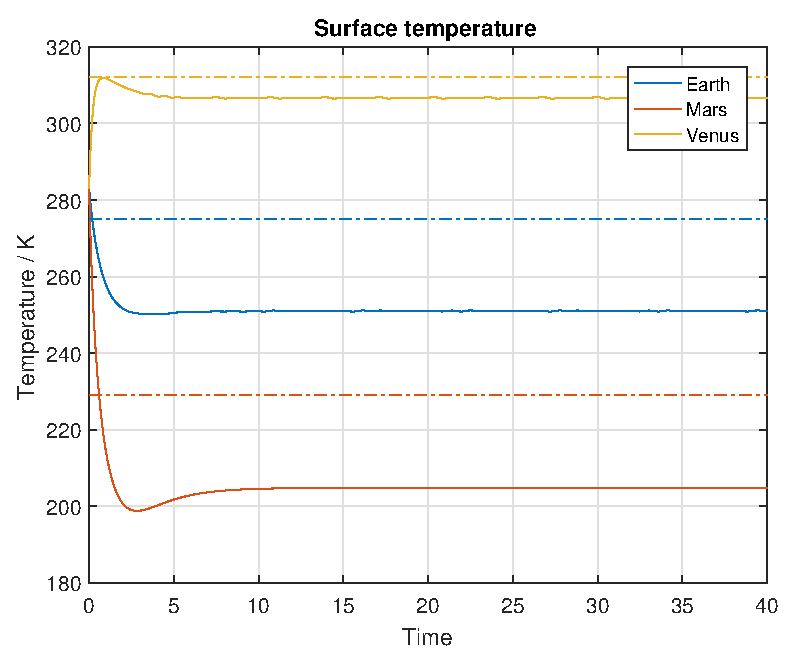
\includegraphics[width=0.9\linewidth]{Matlab/figures/surfaceTemperature.eps}
		\end{figure}
\end{frame}

\subsection{Luftfeuchtigkeit}
\begin{frame}
	\frametitle{Luftfeuchtigkeit}
		\begin{figure}
			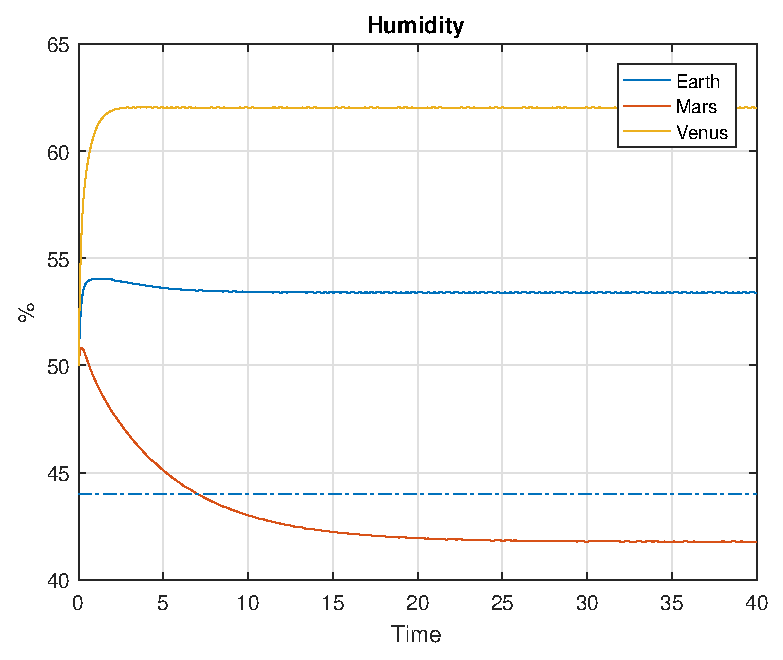
\includegraphics[width=0.9\linewidth]{Matlab/figures/humidity.eps}
		\end{figure}
\end{frame}

\subsection{Wolkenabdeckung}
\begin{frame}
	\frametitle{Wolkenabdeckung}
		\begin{figure}
			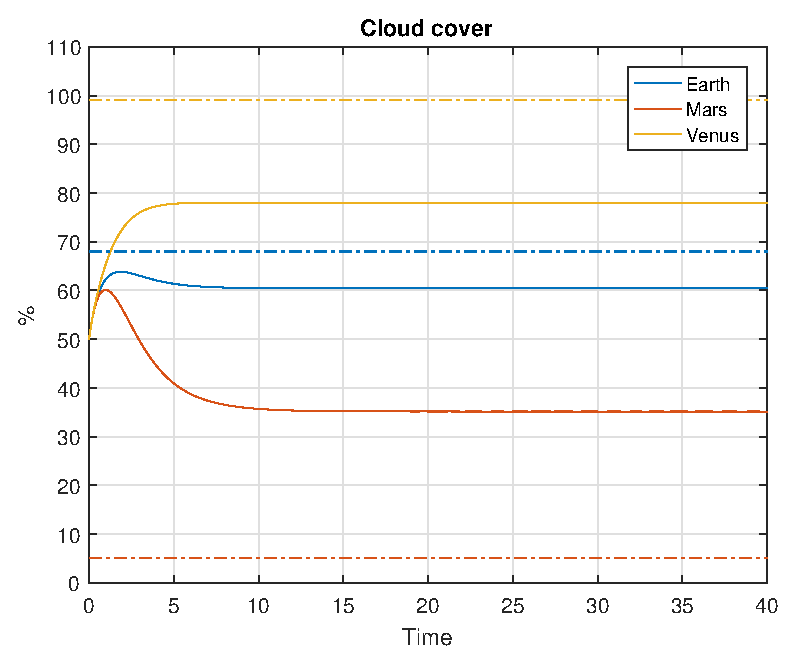
\includegraphics[width=0.9\linewidth]{Matlab/figures/cloudCover.eps}
		\end{figure}
\end{frame}

\subsection{Albedo}
\begin{frame}
	\frametitle{Albedo}
		\begin{figure}
			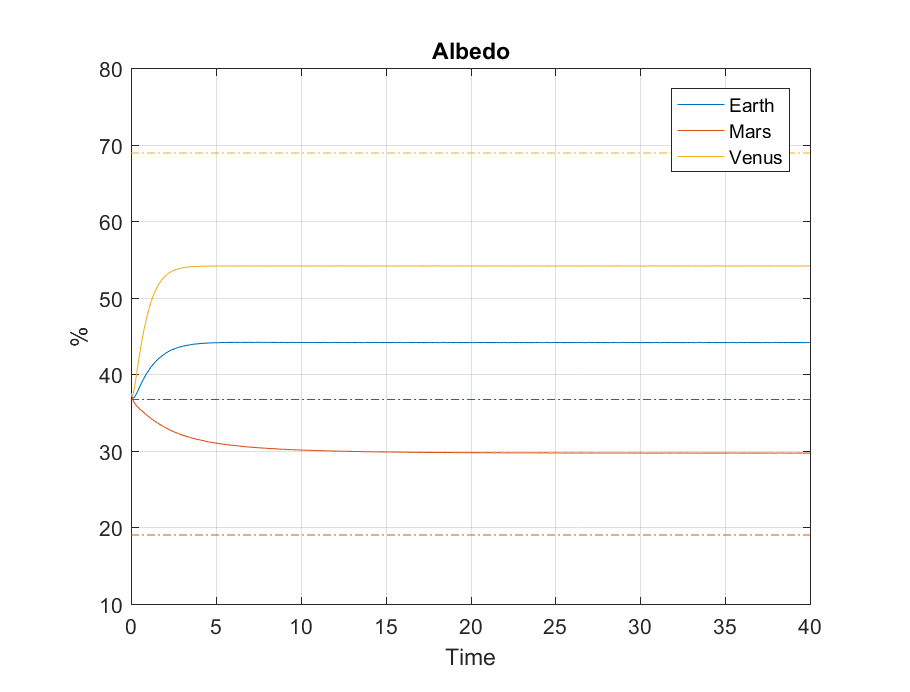
\includegraphics[width=0.9\linewidth]{Matlab/figures/albedo.eps}
		\end{figure}
\end{frame}

\section{Fazit}
\begin{frame}
\frametitle{Fazit}
\begin{itemize}

	\item[$\bullet$] Ergebnisse gleichen dem heutigen status
	\item[$\bullet$] Extremes Klima von Mars \& Venus vermutlich prädestiniert
	
	\vspace{5mm}
	
	\item[$\bullet$] Ergebnisse nur mit Vorsicht zu geniessen	
	\begin{itemize}
		\item[-] Nur Wasser simuliert
		\item[-] Andere Treibhausgase vernaächlässigt
		\item[-] Chemische und Physikalische Vorgänge bei extremen Temperaturen
	\end{itemize}

	
\end{itemize}
\end{frame}

\section{Nächste Schritte}
\begin{frame}
\frametitle{Nächste Schritte}
\begin{itemize}

	\item[$\bullet$] Modell ausbauen
	\begin{itemize}
		\item[-] Vereisung
		\item[-] Tag- \& Nachtseite
		\item[-] Rotationsgeschwindigkeit
		\item[-] Mehr athmosphärische Gase
	\end{itemize}
	
\end{itemize}
\end{frame}

\end{document}